\documentclass[12pt, a4paper]{report}
\usepackage[top=1.0in, bottom=1.0in, left=0.8in, right=0.8in]{geometry}
\usepackage{graphicx}
\usepackage{amsmath}
\usepackage{listings}
\usepackage{fancyvrb}

 	
\title{\textbf{EE2703 : Applied Programming Lab \\ Assignment 6 \\ The Laplace Transform}} 
\author{Aditya Nanda Kishore\\ EE20B062} 

\date{\today} % Date for the report

	
\begin{document}
		
\maketitle
\section*{Introduction}
We wish to analyse a given /textbf{Linear Time Invariant Systems} using python.The aim is to
\begin{itemize}
	\item Analyse the given circuit and find the transfer function
	\item Solve laplace equations and plotting them for better understanding of the time response of the laplace transform
	\item Explore Signals Toolbox in Scipy Library
\end{itemize}


\section*{Question 1 - Inverse Laplace Transform}
Importing necessary libraries
\begin{Verbatim}
from pylab import *
import numpy as np
import scipy.signal as sp
\end{Verbatim}
We are given a system that satisfies 

\begin{equation}
  \ddot x + 2.25x = f(t)
\end{equation}
where 
\begin{equation}
  	f(t) = cos(1.5t)e^{-0.5t}u_o(t)
\end{equation}
and laplace transform of the function is given by 
\begin{equation}
  	F(s)	= \frac{s+0.5}{(s+0.5)^2 + 2.25}
\end{equation}
and we have to find x(t), For that we can find X(s) first from the first equation,

\begin{equation}
  	X(s) = \frac{F(s)}{s^2+ 2.25}
\end{equation}
 and defining our t array and using \text{it}{system.impulse} we get x(t), on plotting it we will get such a graph
\begin{Verbatim}
H = sp.lti([1,d], polymul([1,0,2.25],[1,2*w,w**2 + d**2]))
t,x=sp.impulse(H,None, linspace(0,50,501))
plot(t,x)
title('x(t) with decay 0.5')
xlabel('time')
ylabel('x(t)')
show()
\end{Verbatim}

\begin{figure}[!tbh]
   	\centering
   	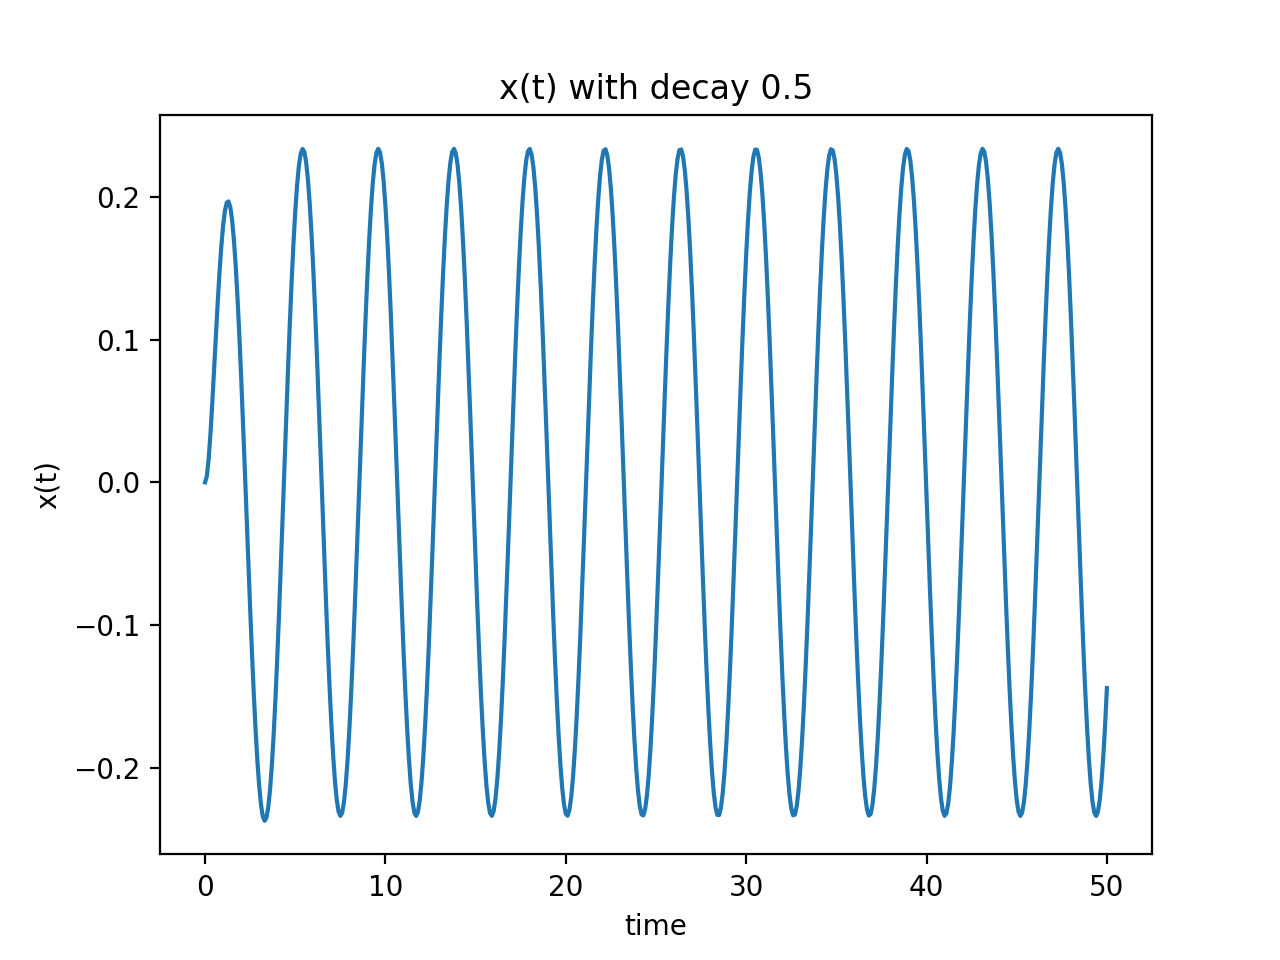
\includegraphics[scale=0.8]{Q1.png}
 \end{figure} 
 
 
 \section*{Question 2 - Decay parameter}

If we carefully observe our \textit{f(s)}, there are two parameters controlling it. One is the frequency of the sinusoid and other is the decay parameter. Let us call them \textit{w} and \textit{d}.Here,

\begin{equation}
  w = 1.5, d = 0.5 
\end{equation}
We are asked to change d to 0.05, so new values are
\begin{equation}
  	w = 1.5, d = 0.05 
\end{equation}
and the new laplace transform of the function is given by 
\begin{equation}
  	F(s)	= \frac{s+0.05}{(s+0.05)^2 + 2.25}
\end{equation}
and 

\begin{equation}
  	X(s) = \frac{F(s)}{s^2+ 2.25}
\end{equation}
Thus new x(t) would be
\begin{Verbatim}
d = 0.05
H = sp.lti([1,0.05], polymul([1,0,2.25],[1,0.1,2.2525]))
t,x2=sp.impulse(H,None, linspace(0,50,501))
plot(t,x2)
title('x(t) with decay 0.05')
xlabel('time')
ylabel('x(t)')
show()

\end{Verbatim}

\begin{figure}[!tbh]
   	\centering
   	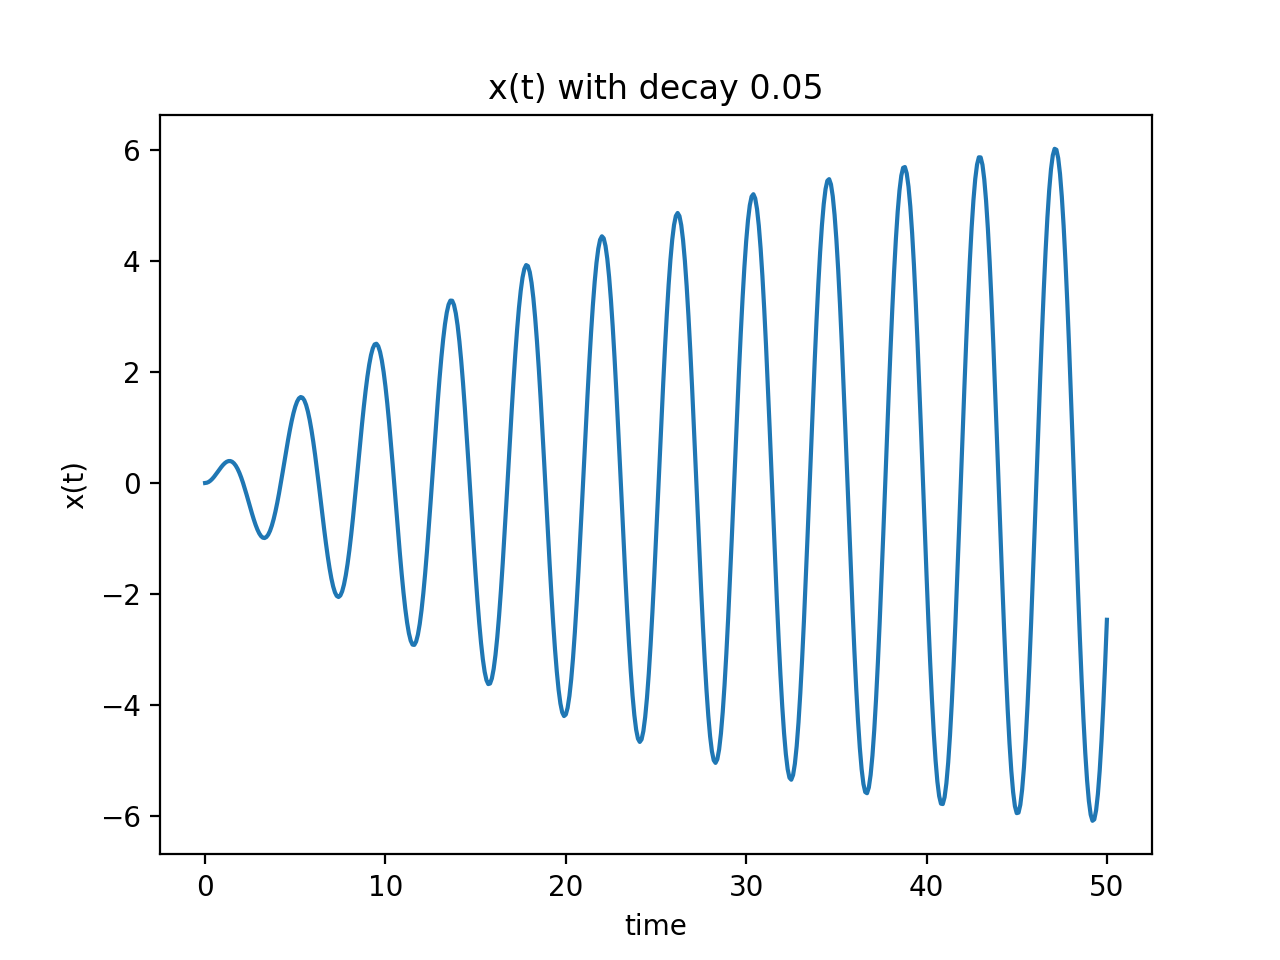
\includegraphics[scale=0.85]{Q2.png}
 \end{figure} 
 
 We can see that after decreasing decay parameter by 10 times, amplitude is just boosting up and up.
 
  \section*{Question 3 - Frequency parameter of the Input}
Let's find natural frequency of the system from the equation of the system

 \begin{equation}
  \ddot x + (\omega_o)^2x = f(t)
\end{equation}
so,comparing it with given values
 \begin{equation}
  \omega_o = 1.5
\end{equation}

Now we change the frequency of the input from 1.4 to 1.6 and check how the graphs are changing

\begin{Verbatim}
transfer_function = poly1d([1,0,2.25])
t=linspace(0,100,1001)\
w = 1.4
figure(0)
for i in range(5):
    u= np.cos(w*t)* np.exp(-d*t)
    H = sp.lti([1,d], polymul([1,0,2.25],[1,2*w,w**2 + d**2]))
    t,y,svec=sp.lsim(H,u,t)
    w += 0.05
    subplot(2,3,i+1)
    plot(t,y)
    title(f'w = {w-0.05}')
    xlabel('time')
    ylabel('x(t)')

show()
\end{Verbatim}

\begin{figure}[!tbh]
   	\centering
   	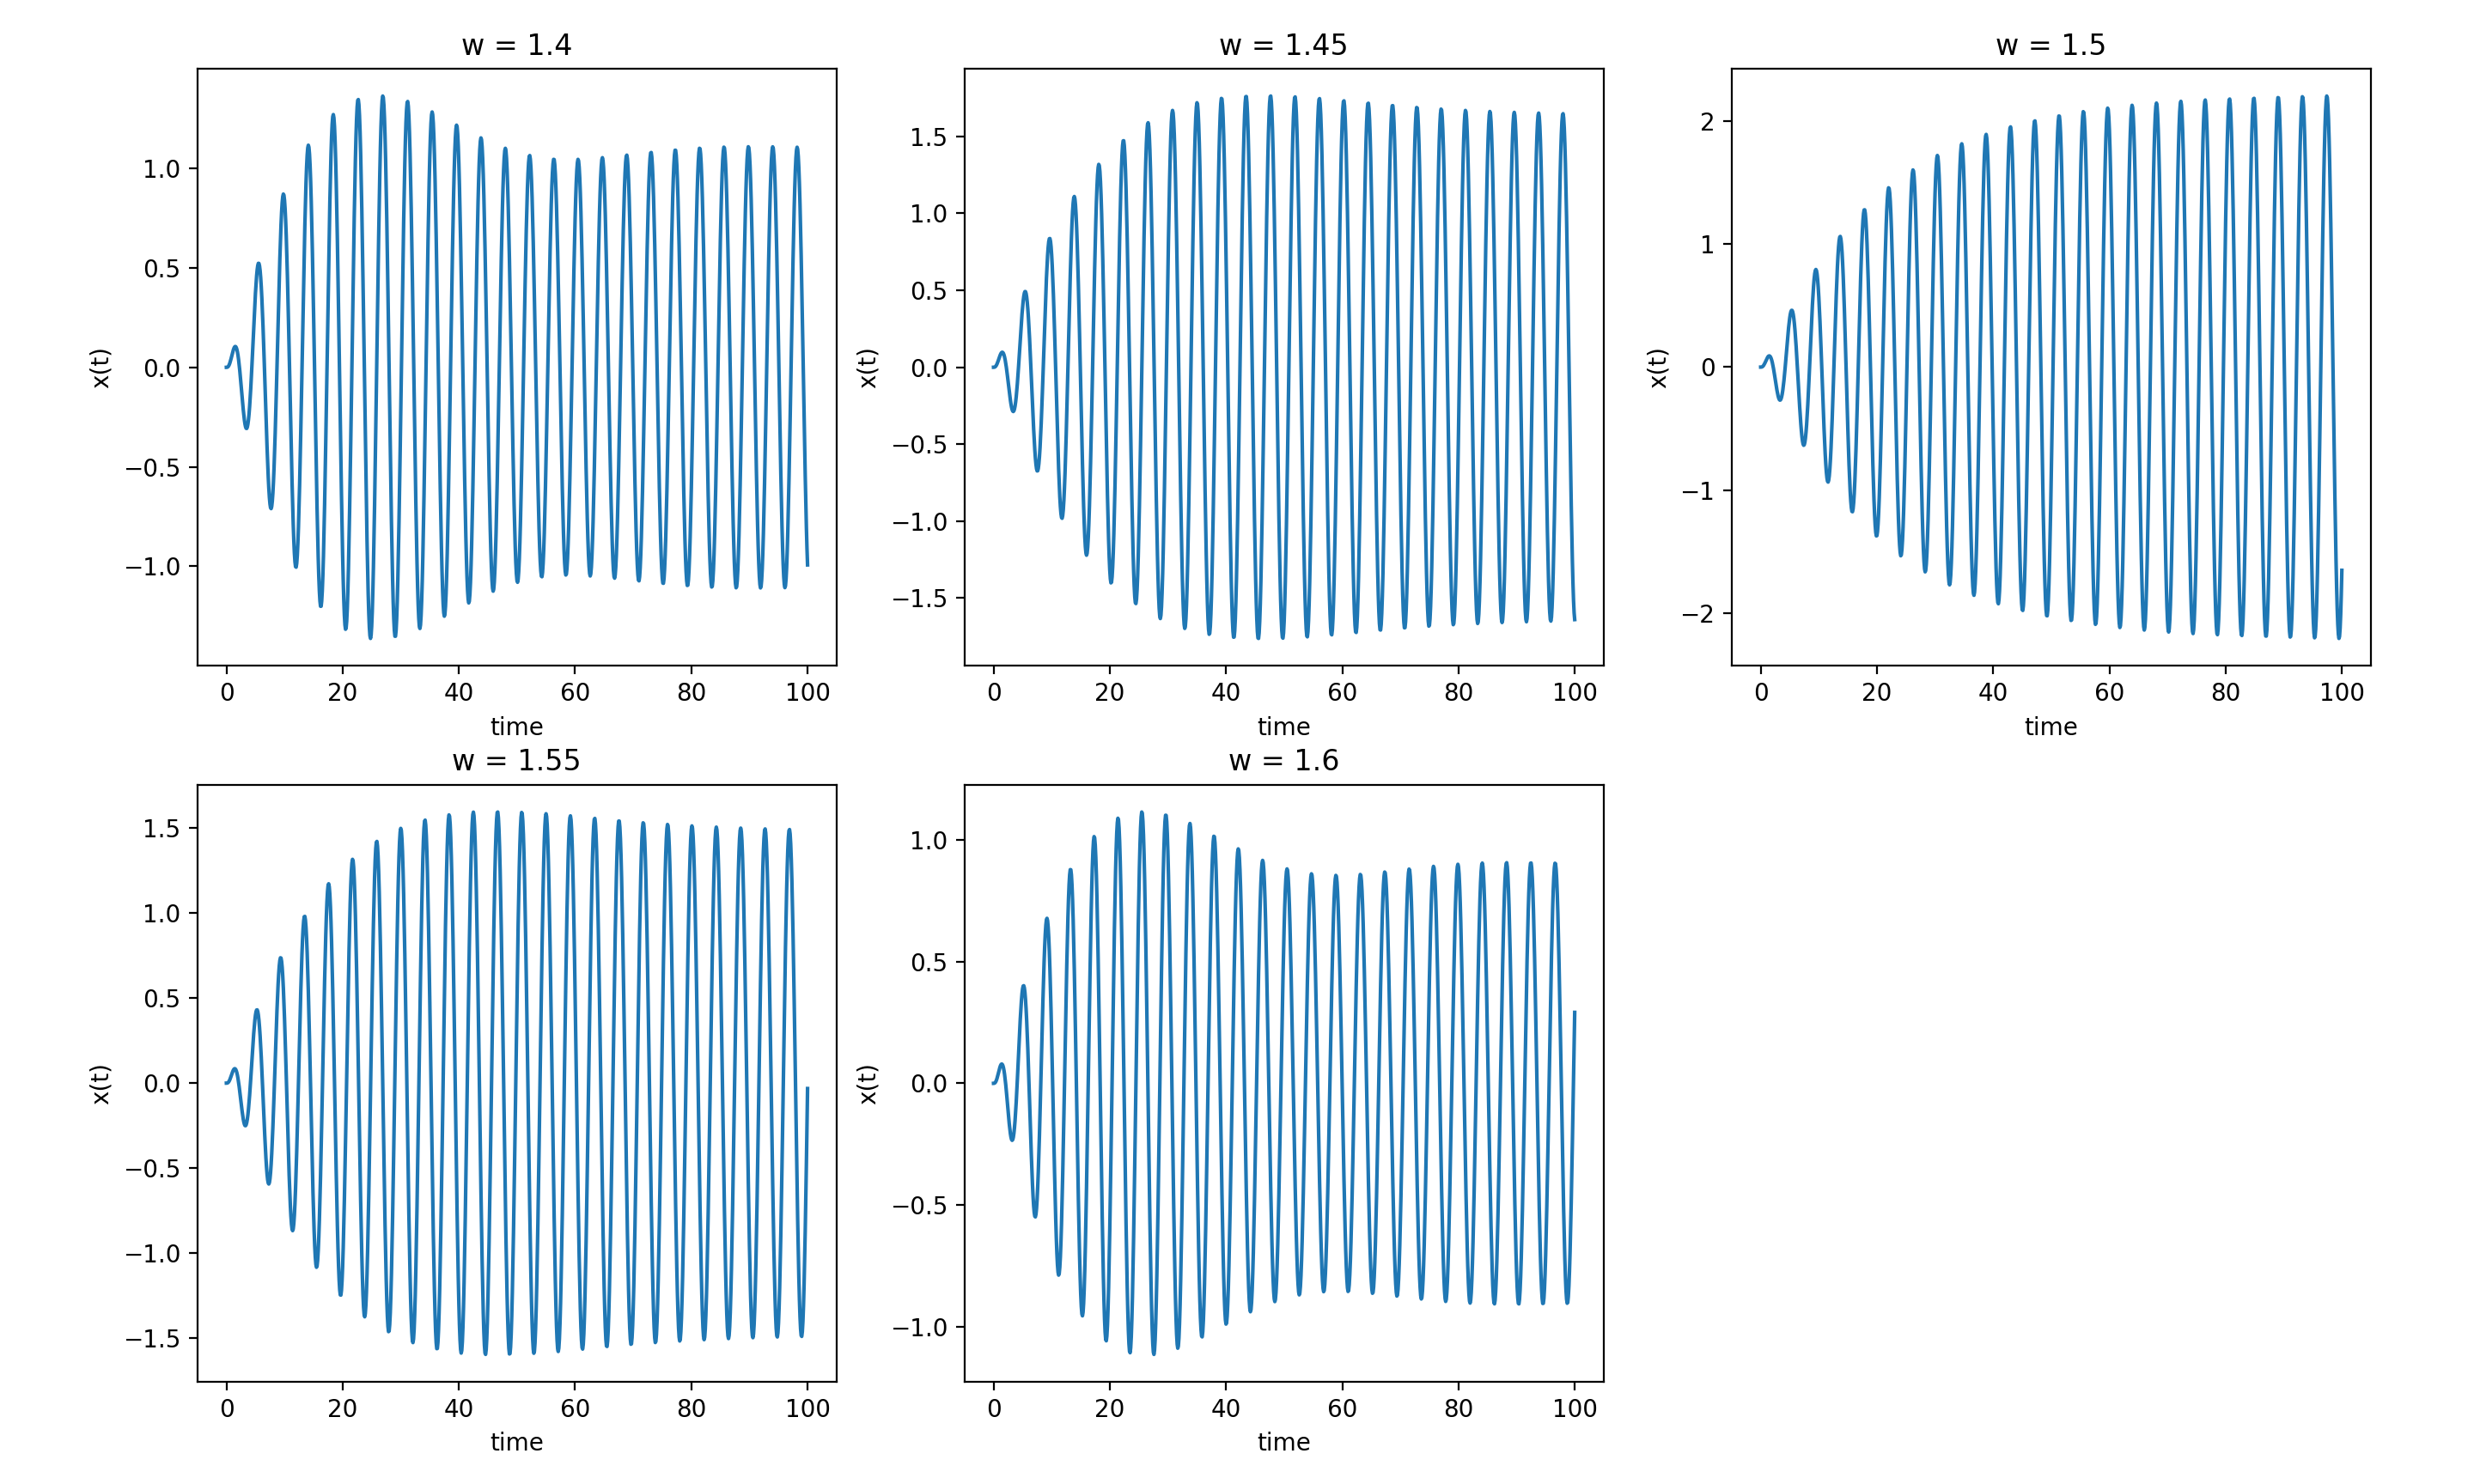
\includegraphics[scale=0.5]{Q3.png}
 \end{figure} 
 
 We can see that at $\omega = 1.5$, the amplitude is growing without a bump and settling naturally unlike other values of $\omega $. It's because 1.5 is also the natural frequency of the system.This is the case of resonance here.


 \section*{Question 4 - Coupled Spring Problem}
 Given equations are

 \begin{equation}
  \ddot x + x - y = 0
\end{equation}
\begin{equation}
  \ddot y + 2(y- x) = 0
\end{equation}

and initial conditions are also given as
\begin{equation}
  \ddot x(0) = 1, \dot x(0) =  \dot x(0) = y(0) = 0
\end{equation}
	
Now, substituting for y from the first equation into the second and solving for x, we get
\begin{equation}
  \ddddot x + 3 \ddot x + x = 0
\end{equation}

Using initial equations, in Laplace domain, equations for x and y are
\begin{equation}
  X(s)= \frac{s^2+2}{s^3+3s}
\end{equation}

\begin{equation}
  Y(s)= \frac{2}{s^3+3s}
\end{equation}



So, time responses are
\begin{Verbatim}
figure(1)
Y = sp.lti([2], [1,0,3,0])
t,y=sp.impulse(Y,None, linspace(0,20,201))
plot(t,y)
X = sp.lti([1,0,2], [1,0,3,0])
t,x = sp.impulse(X,None, linspace(0,20,201))
plot(t,x)
xlabel('time')
legend(['y(t)', 'x(t)'])
show()
\end{Verbatim}

\begin{figure}[!tbh]
   	\centering
   	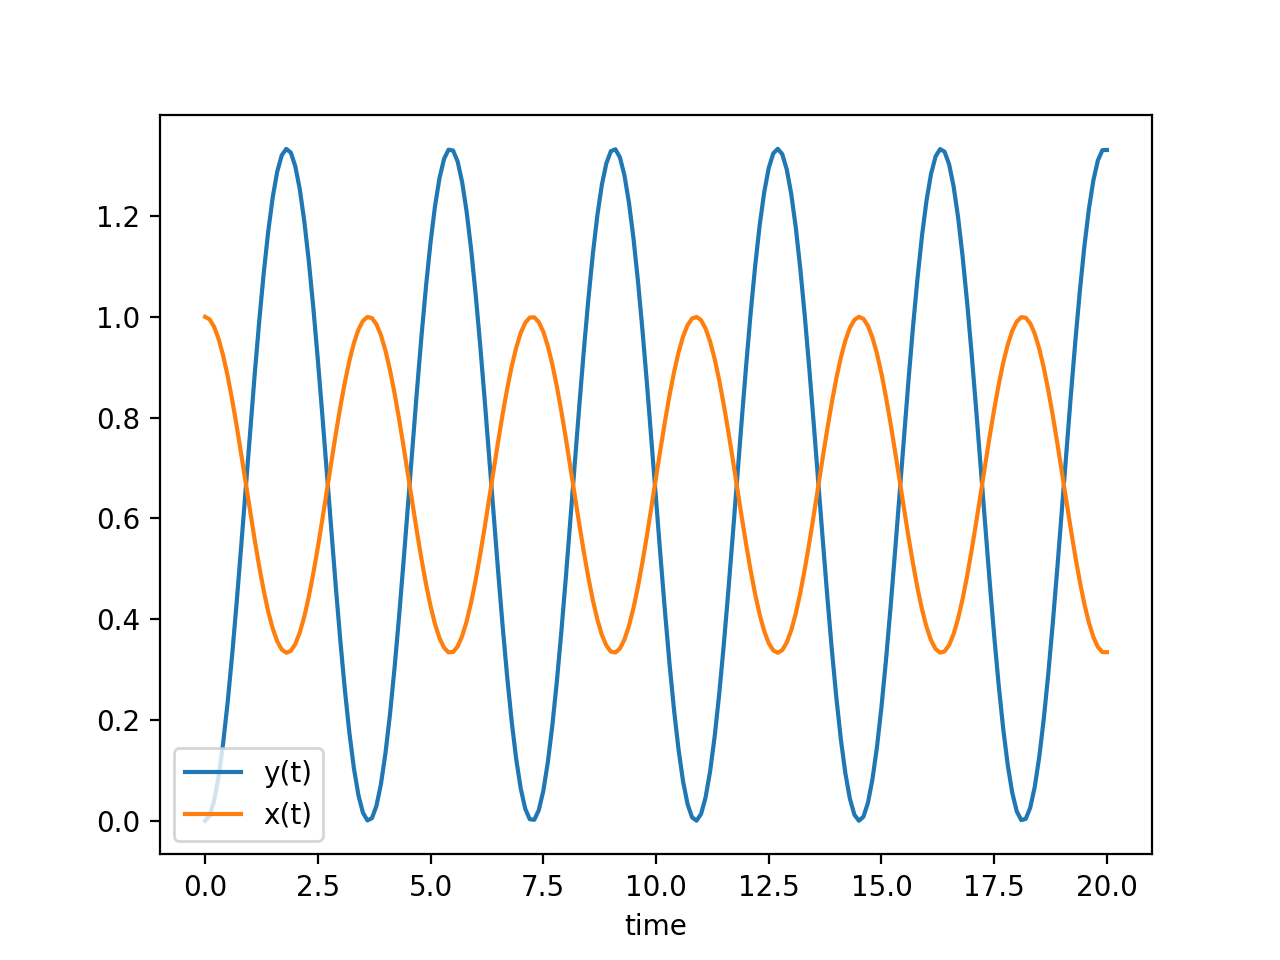
\includegraphics[scale=1]{Q4.png}
 \end{figure} 



\section*{Question 5 - Low pass RLC filter}
Solving the circuit we get 
\begin{equation}
  V_o = \frac{V_i}{R + sL + \frac{1}{sC}} * \frac{1}{sC}
\end{equation}

which implies transfer function is
\begin{equation}
  H = \frac{1}{10^{-12}s^2 + 10^{-4}s + 1}
\end{equation}

So,Plotting Magnitude and Phase response of the System we get
\begin{Verbatim}
figure(2)
H5 = sp.lti([1], [10^{-12} , 10^{-4}, 1])
W,S,phi=H5.bode()
subplot(1,2,1)
xlabel('frequency')
ylabel('Magnitude')
title('Magnitude plot of Steady State Response')
semilogx(W,S)
subplot(1,2,2)
semilogx(W,phi)
xlabel('frequency')
ylabel('Phase')
title('Phase plot of Steady State Response')
show()

\end{Verbatim}

\begin{figure}[!tbh]
   	\centering
   	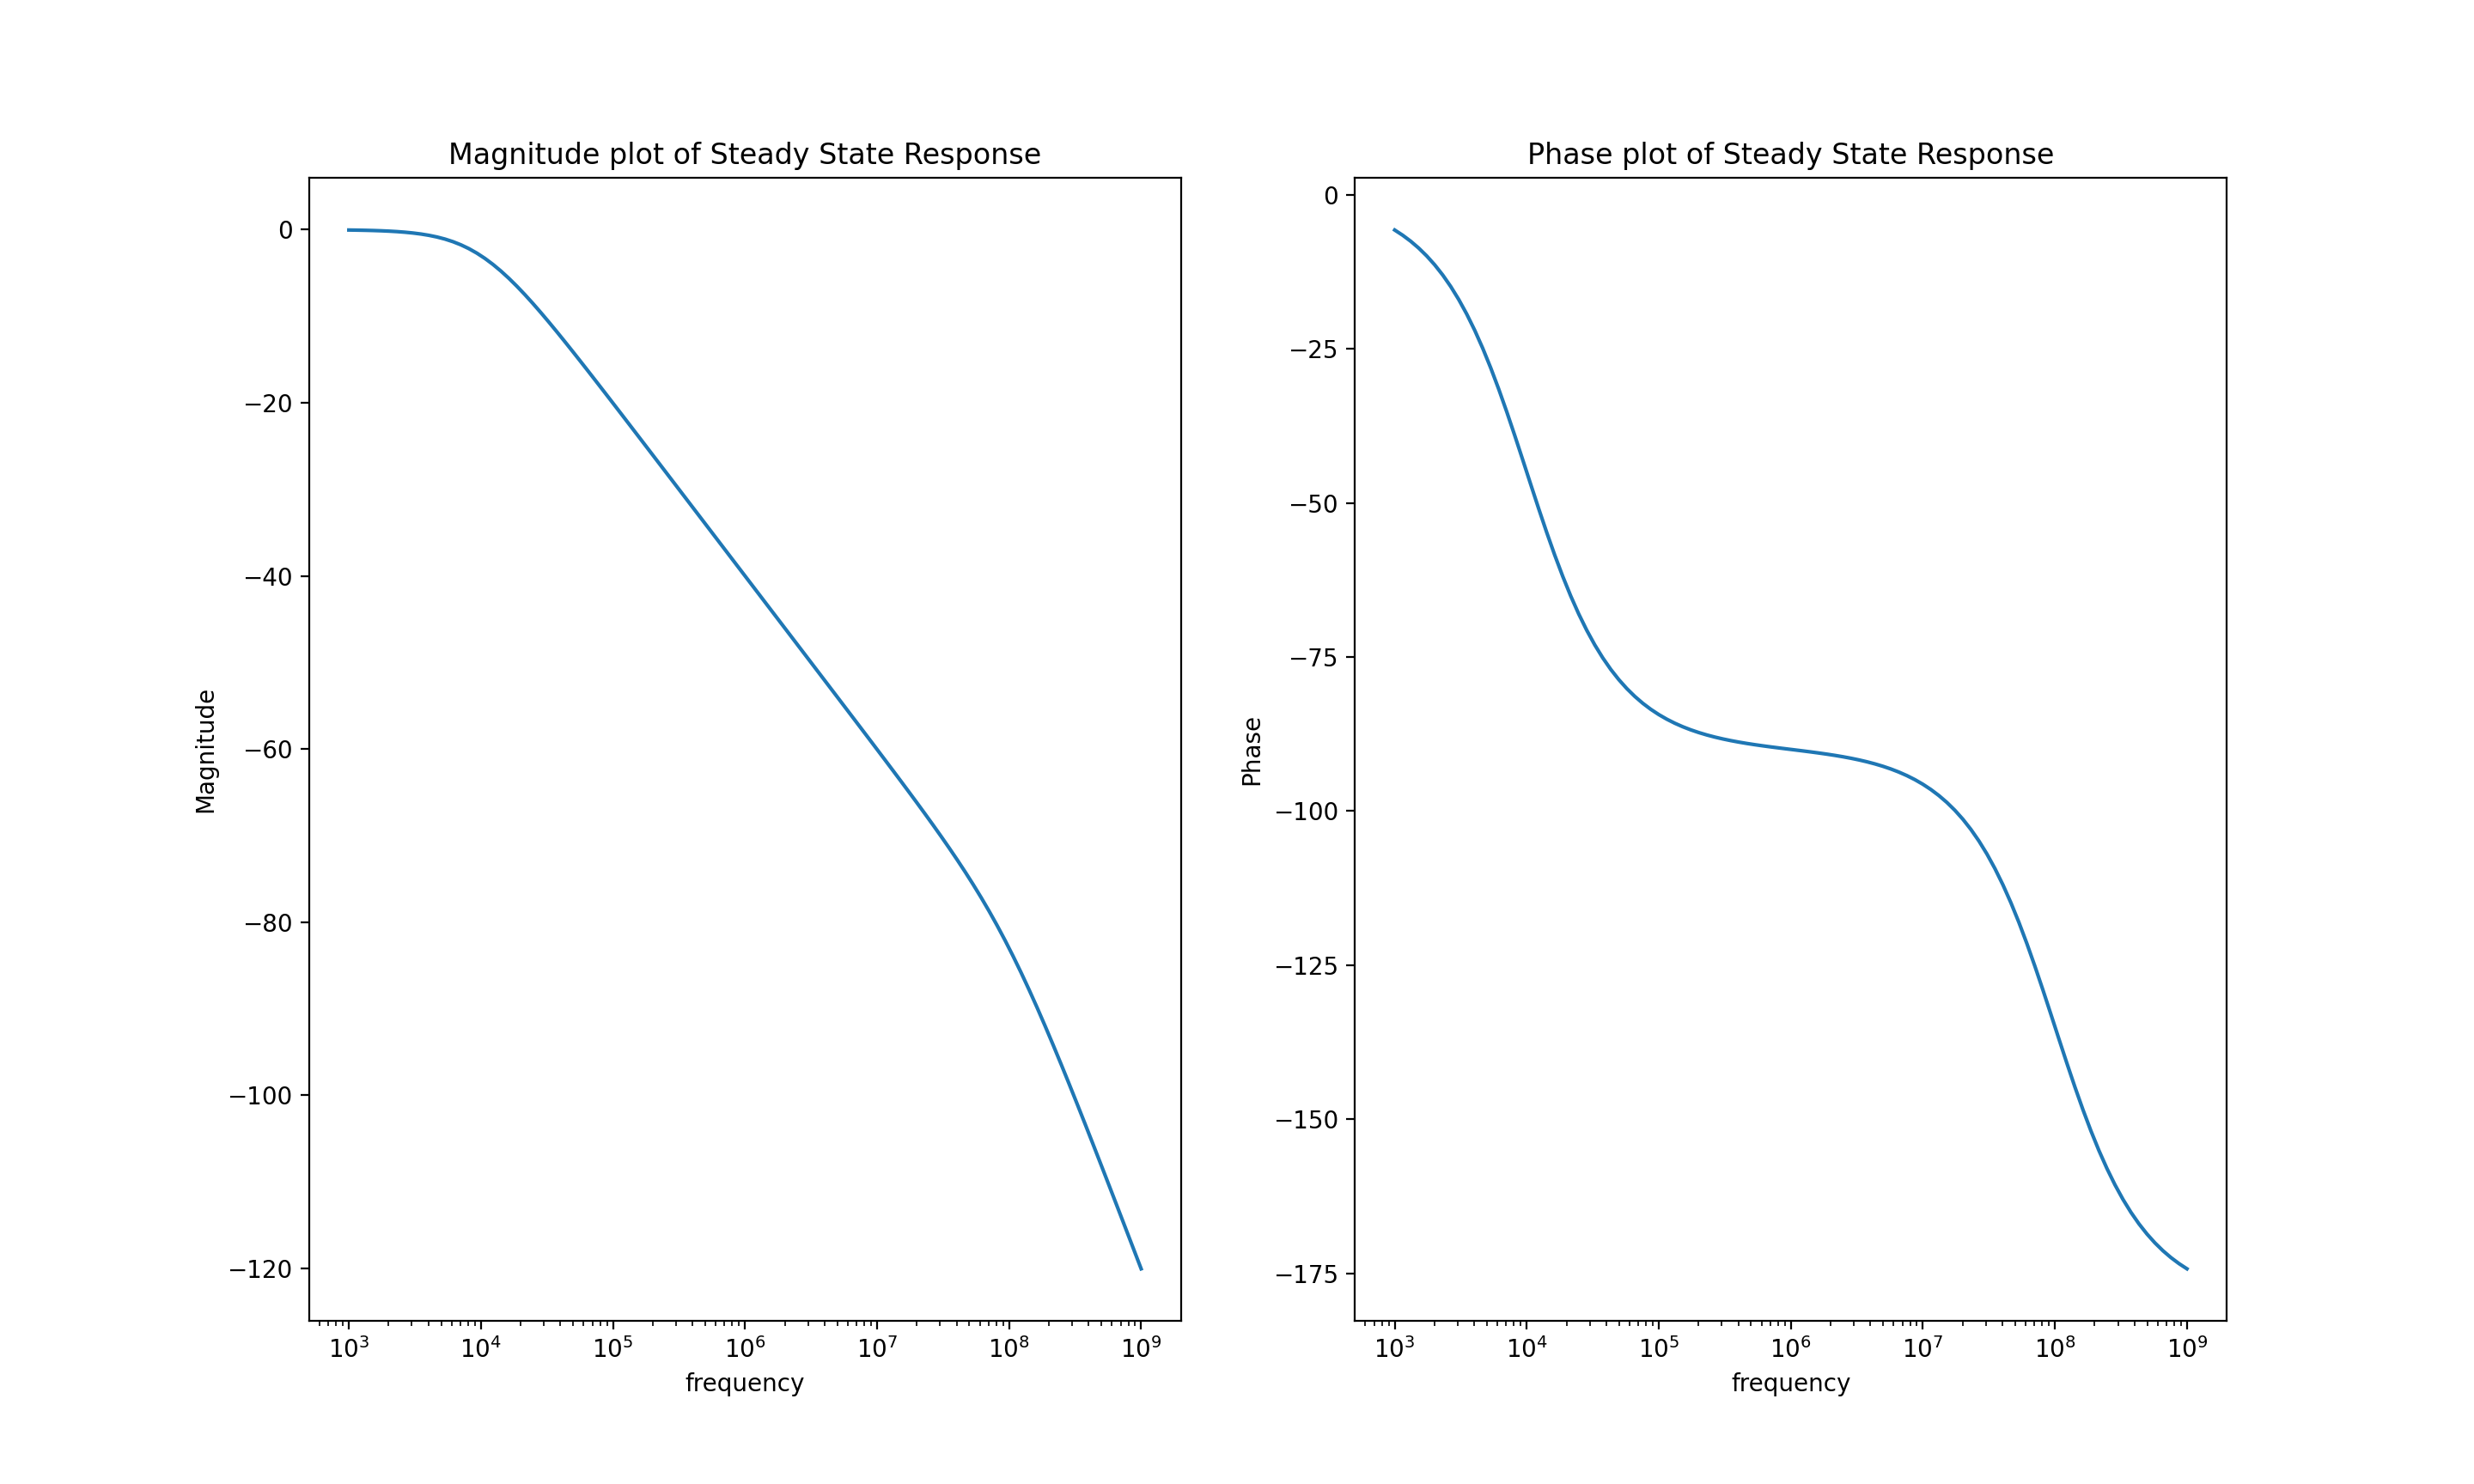
\includegraphics[scale=0.5]{Q5.png}
 \end{figure} 
 
 
 So, It is clear that this is an RLC low pass filter from the bode plot.
 \section*{Question 6 - RLC Low Pass filter with super-positioned input }

I defined the function and plotted two plots with different timescales to analyse short term response and long term response

\begin{Verbatim}
figure(3)
subplot(1,2,1)
t = linspace(0,10**-2,10**4)
Vi = np.cos(1000*t) - np.cos(10**6 * t)
t,Vo_long,svec=sp.lsim(H5,Vi,t)
plot(t, Vo_long)
xlabel('time')
ylabel('Voltage')
title(r'$V_o$ long term response')
subplot(1,2,2)
t_small = linspace(0, 30* (10**-6), 301)
Vi = np.cos(1000*t_small) - np.cos(10**6 * t_small)
t,Vo_small,svec=sp.lsim(H5,Vi,t_small)
plot(t, Vo_small)
xlabel('time')
ylabel('Voltage')
title(r'$V_o$ short term response')
show()
\end{Verbatim}

\begin{figure}[!tbh]
   	\centering
   	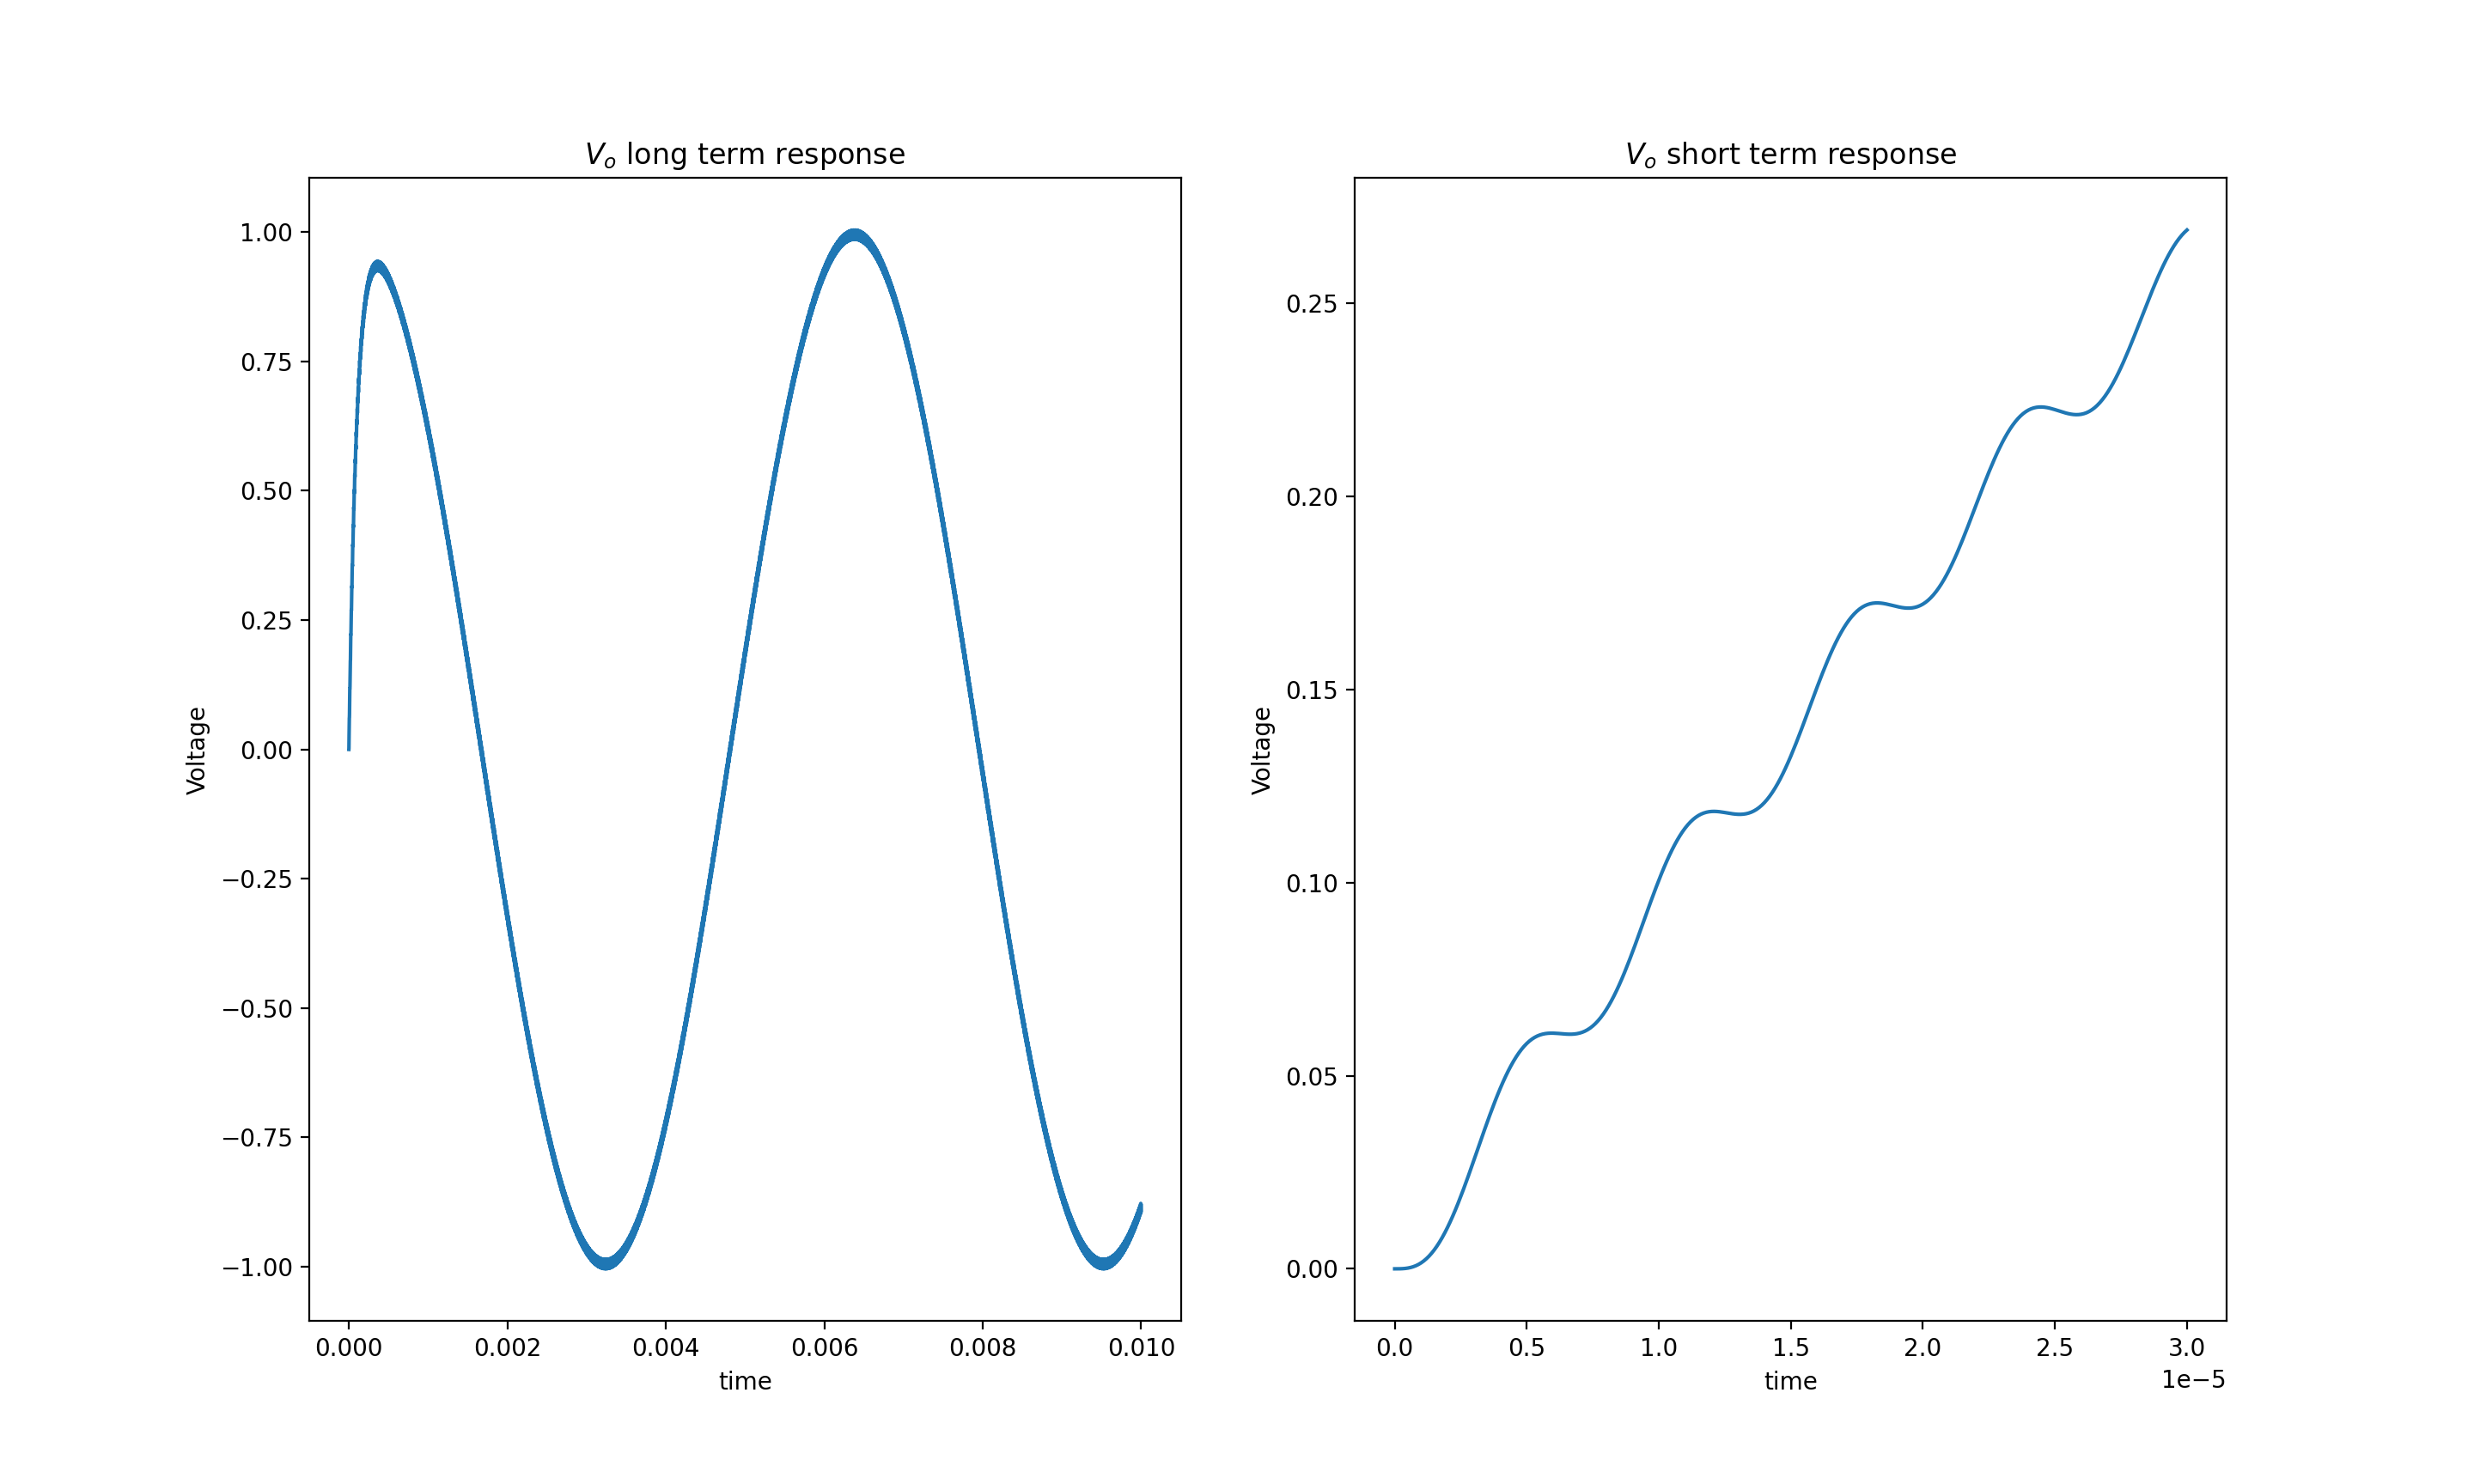
\includegraphics[scale=0.5]{Q6.png}
 \end{figure} 
 

From Bode plot, It is clear that it is a low pass RLC filter, with the low frequency component $10^3 rad/sec$ close to the  $\omega_{3db}$ . It's response has a higher contribution in output than the high frequency component in long run as it is highly attenuated (From Bode plot, we can see that it's close to $-40db$ at $\omega = 10^6 rad/sec$  ) at the higher frequency. Hence, in short time we can see the ripples, as the higher frequency component is not yet attenuated much and contributes to the output. In long time the ripples are lost as it is mostly the solution of the lower frequency component of the input.



\section*{Conclusions}
\begin{itemize}
	\item \textbf{scipy.signal} is a useful toolkit to play around with signals and transfer functions
	\item I understood the low pass RLC filter's working in a much better fashion with the help of accurate plots.
	\item I understood how LTI systems can be solved easily using scipy library
	\item I solved the coupled spring problem and plotted the outputs to understand that the springs will have different oscillation amplitudes based on their $k$ values.
	\item I also understood how forced response can affect a spring system by varying $\omega$ and $d$. With a decrease in d, there will be less decay and output goes to a much higher value, and when input's frequency matches natural frequency of the system we can notice the resonance condition and also the output's peaks increase in a much smoother fashion that that of other $\omega's$.
	
\end{itemize}


\end{document}